\documentclass[conference,a4paper]{IEEEtran}
\IEEEoverridecommandlockouts

\usepackage{cite}
\usepackage{amsmath,amssymb}
\usepackage{graphicx}
\usepackage{array}
\usepackage{booktabs}
\usepackage{url}
\usepackage{tikz}
\usetikzlibrary{positioning,fit,arrows.meta,calc}

\begin{document}

\title{AI Gateways for EuroHPC AI Factories and Antennas: A Functional Reference Model, Technology Landscape and the SAIFA Case%
\thanks{This work has received funding from the European High Performance Computing Joint Undertaking (JU) under Grant Agreement No.~101263280 (SAIFA).}}

\author{
\IEEEauthorblockN{Aleksandra Stojanovi\'c}
\IEEEauthorblockA{\textit{School of Electrical Engineering} \\
\textit{University of Belgrade}\\
Belgrade, Serbia \\
sa230234d@student.etf.bg.ac.rs}
\and
\IEEEauthorblockN{Dimitrije Pe\v{s}i\'c}
\IEEEauthorblockA{\textit{School of Electrical Engineering} \\
\textit{University of Belgrade}\\
Belgrade, Serbia \\
pd230014d@student.etf.bg.ac.rs}
\and
\IEEEauthorblockN{Zaharije Radivojevi\'c}
\IEEEauthorblockA{\textit{School of Electrical Engineering} \\
\textit{University of Belgrade}\\
Belgrade, Serbia \\
zaki@etf.rs}
}

\maketitle

\begin{abstract}
The EuroHPC AI Factories initiative has created a European network of AI-optimised supercomputing centres, extended by AI Factory Antennas that serve countries without large-scale AI infrastructure. As a result, a user may meet several access layers at once: EuroHPC access calls, the EuroHPC Federation Platform, the front offices of individual AI Factories, national Antennas and the AI-on-Demand Platform. This paper analyses this access landscape and proposes a functional reference model for an \emph{AI gateway}, i.e., the user-facing integration and control layer through which an AI Factory or Antenna exposes compute, data, models, workflows, training and support. Ten functional areas are defined and elaborated, the role differences between Factories and Antennas are discussed, and each area is mapped to candidate open-source components together with a two-step selection method. The model is illustrated by the design of the gateway of the Serbian AI Factory Antenna (SAIFA), which is linked with the Pharos and IT4LIA AI Factories.
\end{abstract}

\begin{IEEEkeywords}
AI Factory, AI Factory Antenna, AI gateway, EuroHPC, federation, high-performance computing, MLOps, science gateway.
\end{IEEEkeywords}

\section{Introduction}

Access to large-scale computing has become a precondition for competitive AI research and innovation. The EuroHPC Joint Undertaking (JU) responded by launching the AI Factories initiative. By October 2025, 19 AI Factories had been selected, each built around an AI-optimised supercomputer and offering data, model development, training and expert support services~\cite{eurohpc_aif,eurohpc_six_aif}. In the same month, 13 AI Factory Antennas were selected to extend these services to further countries, each linked with one or more AI Factories~\cite{eurohpc_antennas,eurohpc_antennas_page}.

This growth brings a practical access problem. Startups, SMEs, researchers and public bodies have to navigate several portals, identities, application procedures and service catalogues before they can run a single experiment. Science gateways have long addressed a similar problem for grid and HPC resources by hiding infrastructure behind community-oriented interfaces~\cite{wilkinsdiehr2007,hudak2018ood}. AI Factories, however, add requirements that classical gateways rarely covered: the full model lifecycle, controlled sharing of data and models, LLM inference, training paths for non-experts, and federation across national and European providers.

This paper makes three contributions: (i)~an analysis of the current AI Factory access landscape, (ii)~a functional reference model for an AI gateway applicable to both AI Factories and Antennas, and (iii)~a technology landscape with a selection method for implementing that model. The design of the gateway of the Serbian AI Factory Antenna (SAIFA)~\cite{cordis_saifa,saifa_d31} serves as a case study.

\section{The AI Factory Access Landscape}

\subsection{AI Factories}
AI Factories are operated by national hosting entities around EuroHPC supercomputers. The JU groups their offer into eight service types: expert engagement; AI consultancy and adoption support; AI-optimised supercomputers and cloud resources; data storage and management; physical co-working hubs; training and skills; AI tools and middleware; and AI software and workflows~\cite{eurohpc_aif_services}. Compute access is granted through EuroHPC access calls, in an \emph{Industrial Innovation} mode with sub-modes for different needs and a \emph{Science and Collaborative} mode~\cite{eurohpc_aif_access}. Each Factory also runs its own front office. For example, the Greek Pharos Factory foresees a dedicated Front Desk as the central point of contact~\cite{eurohpc_pharos}, and the Italian IT4LIA Factory offers its services free of charge to eligible users~\cite{eurohpc_it4lia}.

\subsection{AI Factory Antennas}
Antennas expand and complement the services of existing AI Factories~\cite{eurohpc_antennas_page}. They typically combine a national entry point, smaller-scale local computing, AI sandboxes, sector-oriented support and training, and rely on the linked Factories for large-scale capacity. The linkage forms a many-to-many network: Pharos, for instance, is linked with four Antennas (Pharos-CY, CALYPSO, VEZILKA and SAIFA), whereas the Swiss HEARTS Antenna is linked with four Factories~\cite{eurohpc_antennas}.

\subsection{Cross-cutting platforms}
The EuroHPC Federation Platform (EFP), whose first release was announced in April 2026, offers a single access point to several EuroHPC systems with common authentication and authorisation, harmonised resource allocation and data transfer, and a federated software catalogue. AI Factories are to be incorporated in upcoming releases~\cite{eurohpc_efp}. In parallel, the AI-on-Demand Platform provides European-level discovery of AI assets~\cite{aiod}. Table~\ref{tab:landscape} summarises these layers.

\begin{table}[t]
\centering
\caption{Access layers in the AI Factory ecosystem}
\label{tab:landscape}
\footnotesize
\renewcommand{\arraystretch}{1.1}
\begin{tabular}{@{}p{2.25cm}p{5.75cm}@{}}
\toprule
\textbf{Layer} & \textbf{Main function for the user} \\
\midrule
EuroHPC access calls & Application and evaluation of compute allocations (industrial and scientific modes) \\
EuroHPC Federation Platform & Federated identity, harmonised allocation and data transfer, software catalogue across EuroHPC systems \\
AI Factory front office & Consultancy, expert support, training, data services and compute at a national hosting site \\
AI Factory Antenna & National entry point, local compute and onboarding, routing of users and assets to linked Factories \\
AI-on-Demand Platform & European catalogue and discovery of AI assets \\
\bottomrule
\end{tabular}
\end{table}

The layers are complementary, but none of them offers a lifecycle-oriented working environment that connects national resources, data, models and support with the European layers. That is the role of the AI gateway discussed next.

\section{Functional Reference Model}

We define an AI gateway as a \emph{middleware} layer that accepts user or application requests, applies common identity, policy and metadata rules, and forwards each request to the appropriate connected service (Fig.~\ref{fig:arch}). The gateway is responsible for identity and access enforcement, catalogue and metadata management, request validation and routing, quota checks, status aggregation, audit and provenance. It does not replace schedulers, storage systems, model-serving engines, learning-management systems or partner platforms, and domain logic stays with domain applications or authorised user code. This boundary allows the same model to be instantiated by a Factory, where most requests are served locally, and by an Antenna, where a substantial part is forwarded to linked Factories.

\begin{figure}[t]
\centering
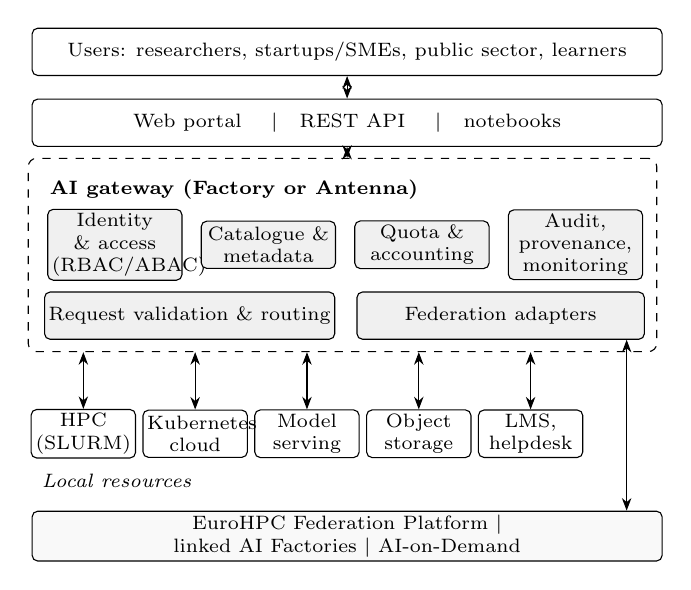
\begin{tikzpicture}[
  font=\scriptsize,
  box/.style={draw, rounded corners=2pt, align=center, minimum height=6mm, inner sep=1.5pt},
  core/.style={box, fill=gray!12},
  >={Stealth[length=1.6mm]}
]
\node[box, minimum width=8cm] (users) at (4,0) {Users: researchers, startups/SMEs, public sector, learners};
\node[box, minimum width=8cm] (portal) at (4,-0.9) {Web portal \quad\textbar\quad REST API \quad\textbar\quad notebooks};
\node[font=\scriptsize\bfseries, anchor=west] (gwt) at (0.1,-1.75) {AI gateway (Factory or Antenna)};
\node[core, text width=1.6cm] (iam)   at (1.05,-2.45) {Identity \& access\\(RBAC/ABAC)};
\node[core, text width=1.6cm] (cat)   at (3.0,-2.45) {Catalogue \&\\metadata};
\node[core, text width=1.6cm] (quota) at (4.95,-2.45) {Quota \&\\accounting};
\node[core, text width=1.6cm] (audit) at (6.9,-2.45) {Audit, provenance,\\monitoring};
\node[core, minimum width=3.65cm] (route) at (2.0,-3.35) {Request validation \& routing};
\node[core, minimum width=3.65cm] (fed)   at (5.95,-3.35) {Federation adapters};
\node[draw, dashed, rounded corners=3pt, fit=(gwt)(iam)(audit)(route)(fed), inner sep=1.5mm] (gw) {};
\foreach \n/\x/\t in {hpc/0.65/{HPC\\(SLURM)}, k8s/2.07/{Kubernetes\\cloud}, serve/3.49/{Model\\serving}, store/4.91/{Object\\storage}, lms/6.33/{LMS,\\helpdesk}}
  \node[box, minimum width=1.3cm, text width=1.22cm] (\n) at (\x,-4.85) {\t};
\node[font=\scriptsize\itshape, anchor=west] at (0,-5.45) {Local resources};
\node[box, minimum width=8cm, fill=gray!5, text width=7.8cm] (aif) at (4,-6.15) {EuroHPC Federation Platform \textbar\ linked AI Factories \textbar\ AI-on-Demand};
\draw[<->] (users) -- (portal);
\draw[<->] (portal) -- (portal |- gw.north);
\foreach \n in {hpc,k8s,serve,store,lms} \draw[<->] (gw.south -| \n) -- (\n);
\draw[<->] (7.55,-3.35 |- fed.south) -- (7.55,-3.35 |- aif.north);
\end{tikzpicture}
\caption{Functional reference model of an AI gateway between users, local resources and the European AI Factory layers.}
\label{fig:arch}
\end{figure}

The functional areas in Table~\ref{tab:func} were derived bottom-up in the SAIFA design (Section~\ref{sec:saifa}) from domain user stories and system use cases. They are, however, formulated so that they apply to any Factory or Antenna. Three requirements cut across all areas: every action is authorised server-side, every artefact carries provenance and version information, and every resource-consuming request is checked against quota before execution.

\begin{table}[t]
\centering
\caption{Functional areas of the reference model}
\label{tab:func}
\footnotesize
\renewcommand{\arraystretch}{1.1}
\begin{tabular}{@{}p{2.1cm}p{5.9cm}@{}}
\toprule
\textbf{Area} & \textbf{Representative capabilities} \\
\midrule
Identity \& access & Institutional (eduGAIN) and EuroHPC sign-in, account linking, RBAC/ABAC, scoped API tokens, revocation \\
Organisations \& projects & Workspaces, membership, roles, resource visibility (private, project, platform, public) \\
Catalogue & Search of models, datasets, workflows, services and courses; source attribution of federated entries \\
Data \& model management & Resumable upload, versioning, model and data cards, review and publication workflow \\
Compute jobs & Job templates, quota reservation, routing to HPC or Kubernetes, status, logs, result retrieval \\
Inference & Authenticated, rate-limited access to served models and LLMs \\
Experiments \& MLOps & Experiment tracking, run comparison, benchmark evaluation, lineage across job, dataset and model \\
Training & Courses, learning paths, preconfigured notebook labs with controlled resources \\
Operations & Monitoring, usage accounting, audit trail, notifications, contextual helpdesk tickets \\
Federation & Catalogue exchange, metadata mapping, identity brokering, cross-factory execution and accounting \\
\bottomrule
\end{tabular}
\end{table}

\begin{table*}[t]
\centering
\caption{Candidate components per layer and gateway-specific integration}
\label{tab:tools}
\footnotesize
\renewcommand{\arraystretch}{1.08}
\begin{tabular}{@{}p{3.0cm}p{7.2cm}p{6.6cm}@{}}
\toprule
\textbf{Layer} & \textbf{Candidates (alternatives)} & \textbf{Gateway-specific integration} \\
\midrule
Portal \& UX & Next.js/React (Nuxt/Vue) & unified UI, backend-for-frontend, tool embedding \\
Identity \& policies & Keycloak (authentik, WSO2 IS); Open Policy Agent (Casbin, Cedar) & role mapping, ABAC attributes, account linking, policy model \\
Notebooks & JupyterHub + KubeSpawner (SlurmSpawner, code-server) & launch from portal, quotas, dataset mount, audit \\
Catalogue \& search & CKAN or Dataverse (DataHub, OpenMetadata); OpenSearch + pgvector & unified catalogue, ACL filtering in index, federation \\
Model registry \& experiments & MLflow (ClearML, Aim) & model cards, approval workflow, access rights \\
LLM inference \& serving & vLLM (TGI, SGLang, Triton); KServe (Ray Serve, BentoML) & API proxy, quotas, routing, audit \\
Fine-tuning & Hugging Face TRL/PEFT (Axolotl, LLaMA-Factory) & approved templates, HPC submission, result registration \\
HPC \& batch & SLURM, Open OnDemand; Kubernetes Jobs (Volcano, Kueue) & HPC bridge, unified job model, SLURM/K8s routing \\
Workflows \& containers & Argo Workflows (Airflow, Flyte); Harbor + Trivy, Apptainer on HPC & workflow templates, image approval and HPC conversion \\
Storage & PostgreSQL, S3-compatible object store (MinIO/Ceph), Valkey & metadata links, lifecycle, retention \\
Observability \& audit & Prometheus, Grafana, Loki, OpenTelemetry; append-only log + WORM archive & correlation with user/job, shared audit events \\
Learning \& support & Moodle (Open edX); Zammad or GLPI & portal links, lab quotas, contextual tickets \\
Lineage & OpenLineage + Marquez & job--dataset--model--result links \\
Federation \& accounting & DCAT/DCAT-AP adapters (CKAN harvester); Waldur as cross-layer option & partner adapters, per-factory accounting \\
\bottomrule
\end{tabular}
\end{table*}

\section{Elaboration of the Functional Areas}

\subsection{Identity, access and collaboration}
Users authenticate through their home institution (e.g., via eduGAIN) or through the EuroHPC identity path, and the gateway links these identities to a single account. Access decisions use roles together with attributes such as organisation, project and data classification~\cite{nist_abac}. Catalogue visibility is separated from artefact access, and access-aware filtering is applied at the search-index level, so that cross-project leakage is prevented by design rather than by the user interface.

\subsection{Catalogue, data and model lifecycle}
Datasets and models follow a draft--review--publish lifecycle. Reviewers' decisions are recorded for audit, and only verified, immutable versions can be served, published or exported. Large transfers are resumable and checksummed. Published assets carry FAIR metadata~\cite{wilkinson2016fair}, which also makes them suitable for exchange with partner catalogues.

\subsection{Compute, inference and MLOps}
Before a job is dispatched, the gateway validates inputs and access and reserves quota. It then routes the job to HPC through SLURM~\cite{yoo2003slurm} or to Kubernetes~\cite{burns2016borg}, and enforces compute-to-data execution where data may not leave a site. Schedulers remain authoritative for queueing; the gateway aggregates status, logs and results into a unified job model, and containers are converted to Apptainer/Singularity images~\cite{kurtzer2017singularity} for HPC. Inference requests pass a proxy that authenticates the caller, checks limits and charges quota before forwarding. Training and evaluation runs are tracked with lineage to datasets, jobs and benchmark versions, and promotion of a model always remains a human decision.

\subsection{Training and support}
Learners use preconfigured notebook labs with read-only data and approved job templates, so they never interact with schedulers directly. Help requests are opened in context, with the relevant job or resource identifiers attached.

\subsection{Federation: Factory versus Antenna}
Federation is where the two roles differ most. A Factory mainly \emph{publishes} its services and assets to the European layers. An Antenna must additionally \emph{broker} its users to one or more linked Factories: it maps identities and metadata, forwards compute-intensive validation to a partner site, returns the results to the originating project, and accounts consumption per Factory. Each partner is integrated through a separate catalogue adapter, e.g., using DCAT~\cite{w3c_dcat3}. Federated entries keep their origin and are never overwritten. Integration starts with read-only or mocked interfaces so that the gateway remains usable when a partner is unavailable. Once AI Factories are added to the EFP~\cite{eurohpc_efp}, gateways should reuse its identity and allocation services rather than duplicate them.

\section{Technology Landscape and Selection}

The guiding principle is \emph{reuse before build, integrate before replace}. Table~\ref{tab:tools} maps each layer to leading open-source candidates, with alternatives in parentheses, and to the integration logic that has to be developed specifically for each gateway. Most candidates are mature projects, e.g., JupyterHub~\cite{kluyver2016jupyter}, MLflow~\cite{zaharia2018mlflow}, vLLM~\cite{kwon2023vllm} and Open OnDemand~\cite{hudak2018ood}. Custom development therefore concentrates on the unified portal, the canonical metadata model, common authorisation and quota rules, audit and accounting, the HPC bridge and federation adapters. Waldur is a notable cross-layer candidate for cataloguing, allocation, accounting and HPC provisioning, but it should be compared against a combination of specialised tools.

Selection proceeds in two steps. First, a candidate must pass the mandatory criteria of its domain. Examples are federation over SAML2 and OIDC to one identity with immediate revocation, ACL filtering at the index level, an inference runtime behind the gateway with quota charged before execution, SLURM abstracted from the user, and new partners added as new adapters. Candidates that pass are then compared on user experience, integration effort, operational complexity, performance and cost, maturity, and compliance (GDPR, data sovereignty, licensing). OSI-approved, self-hostable software is preferred, and paid or source-available dependencies are recorded with an exit option.

\section{Case Study: SAIFA}
\label{sec:saifa}

SAIFA (May 2026--April 2029) is the Serbian Antenna linked with Pharos and IT4LIA~\cite{cordis_saifa}. Its local resources are the PARADOX HPC cluster at the Institute of Physics Belgrade and the AI infrastructure of the Institute for AI Research and Development of Serbia, and it targets four domains: language and culture, energy and manufacturing, health, and environment. The functional areas of Table~\ref{tab:func} were derived from 23 domain user stories, such as AutoML-based flood-prediction digital twins, synthetic genome sequencing data, Serbian hate-speech detection and LLM-driven social-platform simulation, which were generalised into 20 system use cases~\cite{saifa_d31}.

The beta proof-of-concept baseline consists of a web portal, federated identity, a policy module, PostgreSQL with S3-compatible storage, JupyterHub, a managed inference service, SLURM integration through an isolated bridge, and Prometheus/Grafana observability. Each component must demonstrate identity propagation, resource charging, audit recording and graceful behaviour on dependency failure. The beta is due in April 2027 with at least one end-to-end path through identity, discovery, execution and monitoring. Final validation and benchmarking are planned on the Greek and Italian Factories.

\section{Conclusion and Open Challenges}

The AI Factory ecosystem already provides strong compute, service and federation layers, but users still need a lifecycle-oriented gateway that ties them together. The proposed reference model defines such a gateway as an integration and control layer with a clear responsibility boundary, applicable to both Factories and Antennas, and implementable largely from mature open-source components. Open challenges for the ecosystem include identity and allocation alignment with the EFP, accounting across multiple Factories, common metadata profiles for exchanging models and datasets, and data-sovereignty rules for cross-border execution. Future work will report on the SAIFA beta and on interoperability tests with Pharos and IT4LIA.

\bibliographystyle{IEEEtran}
\bibliography{references_v2}

\end{document}
